\section{Firewall Intrusion Detection and Evasion}

\subsection{Overview}

\paragraph{Firewall}
A system protecting or separating a trusted network from an untrusted one. It either permits, denies or proxies data through a network with different levels of trust. = Access control policy between two networks.

This is not enough. Many ports need to be kept open for legitimate applications to run. Evolution messes with legacy firewall technology (P2P. instant messaging, Web 2.0 - multiple functions for single-function port, etc.).

\textbf{Network firewall:} Software appliance running on specific hardware or as a virtual instance. Filters traffic between two or more networks. Protects different network segments.

\textbf{Host firewall:} Layer of software on a host that controls traffic going in and out of a single machine. Protects single host.

\textbf{Stateless firewall:} Examine a packet at the network layer and base decision on packet header information. Application independent and good performance / scalability, but no context.

\textbf{Stateful firewall:} Also keep track of state of network connections and base decision on packet header and session state. More powerful rules are possible but state can be inconsistent / nonexistent (UDP) and explode ((D)DoS).

\paragraph{Filtering Rules}
\begin{itemize}
    \item \textbf{Ingress:} Incoming traffic, low to high security network.
    \item \textbf{Egress:} Outgoing traffic, high to low security network.
    \item \textbf{Default:} Define what to do if no rule matches (accept / reject).
    \item \textbf{Deny Access:} Either silently drop or reject (\textit{ICMP Destination Unreachable}) packet.
\end{itemize}

\paragraph{Next Generation Firewall (NGFW)}
Performs deep packet (payload) inspection and takes application and protocol state into account (on top of typical firewall functions). Allows for powerful rules and application / protocol awareness. Cons: needs to support many application protocols, impacts performance / scalability, deals with inconsistent state (host vs. firewall), etc. %TODO: more? examples?

\paragraph{Web Application Firewall (WAF)}
Protects web-based applications from malicious requests by filtering based on requests / signatures (SQL injection, cross-site scripting, buffer overflow, checking number of form parameters, etc.). Allows for static or dynamic black- / whitelisting. Con: false positive problem.

WAFs are often implemented as a reverse proxy (client outside of internal network) to protect public facing web applications.

\paragraph{Deployment Challenges}
How to protect a large number of hosts / endpoints / network segments.

\begin{itemize}
    \item \textbf{Complexity:} Rules can be complex, thousands of rules per firewall are common, detection between channels is out of sync (mail vs. net vs. proxy).
    \item \textbf{Management:} How to change / remove rules? Who has the permission? What tools?
    \item \textbf{Incentives:} Infrastructure team is paid for providing connectivity and blamed for disruptions and security team is paid to protect and disrupt connectivity...
\end{itemize}

\subsection{Firewall Attack Methods}

\paragraph{IP Source Spoofing}
Spoofing the source IP address. Works for stateless protocols (e.g. UDP, ineffective for TCP).

\paragraph{Artificial Fragmentation}
A fragmented packet might pass a firewall if it's not able to properly reassemble it (e.g. because they're out of sequence). For example, the port number is only in the first fragment. Also works by splitting the attack into multiple packets or overlapping the individual fragments.

\paragraph{Denial of Service}
Firewall state explosion. Need to define a good fallback policy.

\paragraph{Tunneling / Covert Channels}
Creating a capability to transfer information between processes that are not supposed to communicate. For example, putting data in ICMP ping packets or using DNS requests as a channel. Furthermore, attacks can also be performed through a VPN tunnel.

\paragraph{Payload Encodings}
Use different encodings allowed on the protocol / application in use and addition of noise to confuse detection. Different encoding and obfuscation schemes can be combined with noise insertion in millions of ways and encodings are not necessarily unique. Furthermore, undefined or border cases are very effective for detection evasion. There might also be different implementations of decoding on target application vs. detection engine decoding.

%TODO better examples?

E.g.: URL encodings (\% encoding, path character tranformations) or HTML obfuscations (UTF-7 / UTF-16 / UTF-32 character set encoding, chunked encodings, different compression schemas, Base64 encoding, etc.).

\begin{figure}[h]
	\centering
	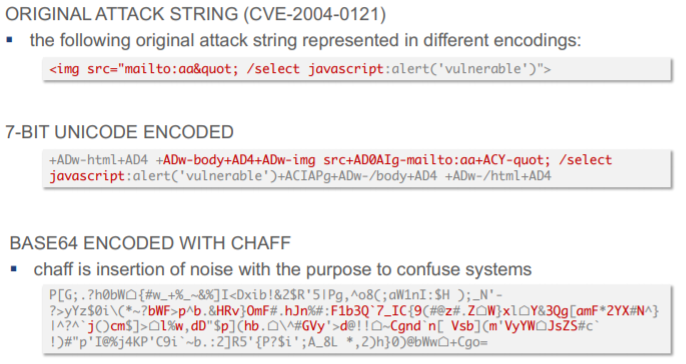
\includegraphics[scale=0.8]{images/911-encodings.PNG}
	\caption{Attack string in different encodings.}
	\label{fig:encoding}
\end{figure}

\paragraph{Firewall Vulnerabilities}
There are several vulnerabilities found in firewall software from security vendors. Firewalls are complex! See examples in Figure \ref{fig:vulnerable}. 

\begin{figure}[h]
	\centering
	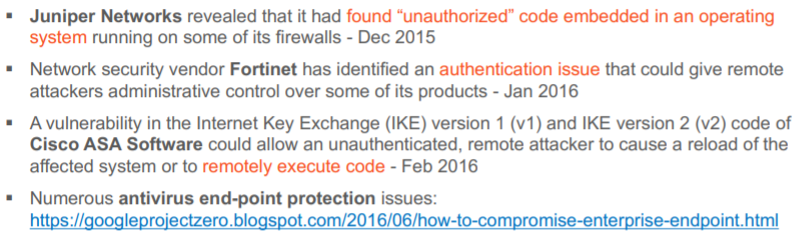
\includegraphics[scale=0.8]{images/911-vulnerable.PNG}
	\caption{Some vulnerabilities found in commercial firewalls.}
	\label{fig:vulnerable}
\end{figure}

\subsection{Intrusion Detection Methods}

\paragraph{Key Features of Intrusion / Attack Detection}
\begin{itemize}
    \item \textbf{Reactive:} System can only detect already known attacks.
    \item \textbf{Proactive:} System can detect known and new, yet unknown attacks.
    \item \textbf{Deterministic:} System always performs the same given the same input. Reason for alert is known.
    \item \textbf{Non-Deterministic:} Detection is fuzzy (heuristics, ML, sandboxing, etc.) and depends on state. Reason for alert is typically not known.
\end{itemize}

\paragraph{Detection Techniques}
See basic detection approaches in Figure \ref{fig:techniques}.

\begin{figure}[h]
	\centering
	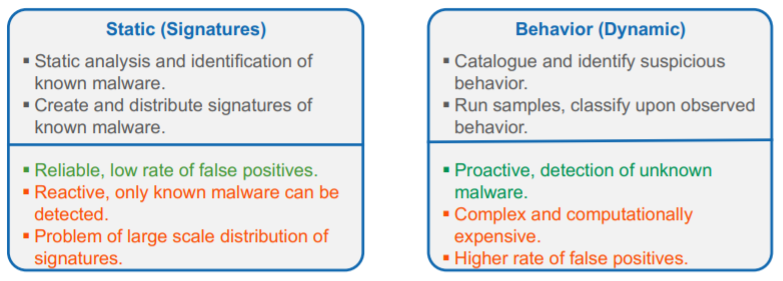
\includegraphics[scale=0.8]{images/911-techniques.PNG}
	\caption{Basic approaches to intrusion detection.}
	\label{fig:techniques}
\end{figure}

Key features include:
\begin{itemize}
    \item \textbf{Protocol Analysis:} Analysis and decoding of protocols. Reassembly and normalization of traffic.
    \item \textbf{Signatures:} Compare attributes of observables to black- / whitelists or to patterns of known attacks / exploits / malware. A signature can be simple groups of checksums / byte arrays or complex hundred lines of code.
    \item \textbf{Sandboxing / Behavior:} Suspicious file is executed within a virtual environment. Specific actions are categorized and labeled as good / bad.
    \item \textbf{Machine Learning:} Recognize complex patterns and make decisions based on data / assumptions formed from previous data. Learn (good vs. bad), extract features, train and test.
    \item \textbf{AI:} not just learning how to solve a specific task very well (ML) but actually learning how to improve itself to solve new previously unknown tasks. Goal: increase chance of success, not accuracy.
\end{itemize}

Signature based approaches will stay and be accompanied by more sophisticated unsupervised ML approaches.

\paragraph{Signature Based Detection}
Core concepts still lie at the heart of all modern detection systems and will continue to be integral for the foreseeable future. Reactive and deterministic. Progression / Sophistication of such systems depend on human signature writers. Bad with mutations / polymorphism. Characteristics:

\begin{itemize}
    \item Able to promptly identify and label a threat.
    \item Different signature systems are used together for more accuracy.
    \item Unique signatures or signature artifacts are created for new threats.
    \item Signature databases / online lookups are frequently updates.
\end{itemize}

Indicators of Compromise (IoC) similar, not a full signature (mostly IPs or file hashes). E.g. Yara Rule.


\textbf{One-Dimensional:} common in all systems, fastest and most efficient way of categorizing a data artifact. Simply a boolean output (good / bad). Doesn't need many resources, is fast and has a low number of false positives but is reactive, needs frequent updates to signatures and uses humans.

\textbf{Two-Dimensional:} regular expression functions and string matching, fundamental for anti-malware / IDS / DLP systems, easily capable of identifying previously known exploits and host enumeration techniques. Low / medium resource requirements, more flexibility with patterns and low false positive rate. Cons: same as above.

\textbf{Multi-Dimensional:} instead of triggering on a single signature, a multi-dimensional signature was created, can label actions as suspicious or bad (sandboxing / network behavioral monitoring). Classify and label threat after a certain threshold of good or bad activities is met. Is partially proactive and more efficient / effective than above approaches.

\paragraph{Sandboxing Based Detection}
Basically running malware in a detonation chamber by examining / monitoring runtime behaviour of a sample and comparing behavior against a list / rules previously developed in a lab or via machine learning (behavior classification - no humans!). Is proactive and mostly deterministic. 
Doesn't require updates to signatures. Cons: resource intensive, high latency and difficult to scale.

\paragraph{Limitations of Intrusion Detection}
\begin{itemize}
    \item Unable to inspect encrypted traffic.
    \item High number of false positives.
    \item Packet capturing and analysis at high link speed (tens of Gbits/s).
    \item Minimize latency introduced by inspection engine.
    \item Application level attacks (JavaScript, etc.).
    \item Policy / signature management.
\end{itemize}

\paragraph{Accuracy vs. Precision}
For decision making (block/pass) the consistency of accuracy is most important. Accurate detection is very challenging (balance zero FN and zero FP). 

%TODO see examples p. 59!! Sensitivity vs. specificity stuff

\textbf{Accuracy:} how close is the measured value to target value (bias).

\textbf{Precision:} Values of repeated measurements are clustered and have little scatter. Can be far away from target value (variance).

\begin{figure}[h]
	\centering
	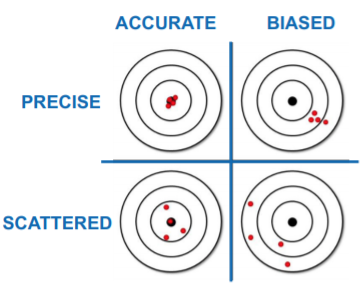
\includegraphics[scale=0.6]{images/911-accprec.PNG}
	\caption{Accuracy vs. precision.}
	\label{fig:accprec}
\end{figure}

\begin{figure}[h]
	\centering
	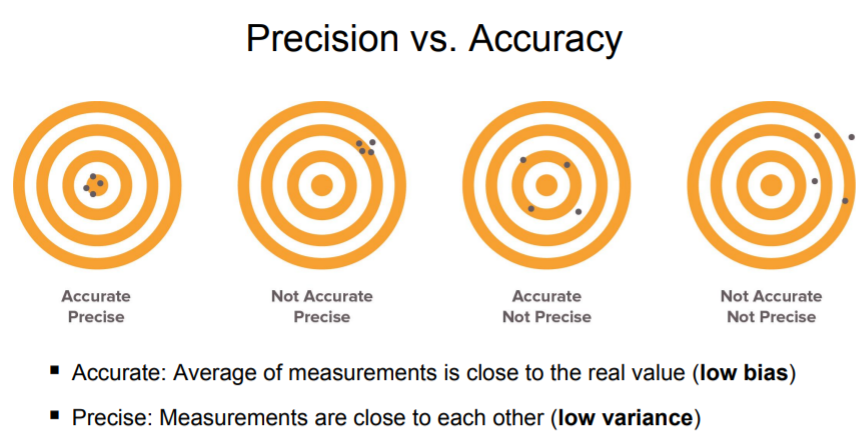
\includegraphics[scale=0.6]{images/911-another.PNG}
	\caption{Another accuracy vs. precision.}
	\label{fig:another}
\end{figure}

\begin{figure}[h]
	\centering
	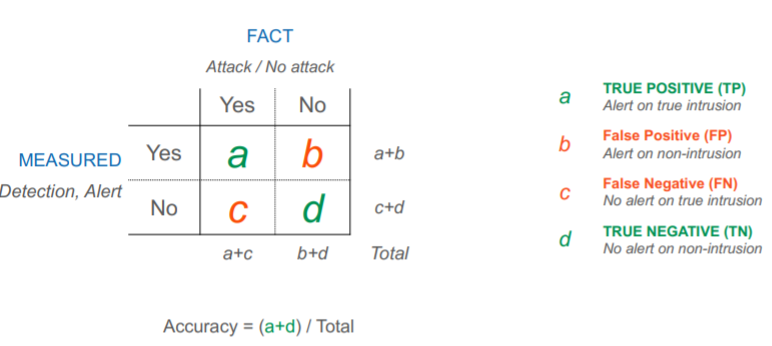
\includegraphics[scale=0.8]{images/911-positives.PNG}
	\caption{Accuracy and type of measurements.}
	\label{fig:positives}
\end{figure}

\paragraph{Sensitivity vs. Specificity}
Sensitivity measures the proportion of positives that are correctly identified (TP / all positives resp. FN + TP). Specificity measures the proportion of negatives that are correctly identified (TN / all negatives resp. FP + TN).

\paragraph{Detection Performance}
\begin{itemize}
    \item Accurate detection is very challenging when rate of attacks is very low.
    \item Different detection techniques achieve different sensitivity and specificity.
    \item Use a combination of diverse tests to increase precision.
    \item Context is important (host vs. network based detection).
\end{itemize}

\begin{figure}[h]
	\centering
	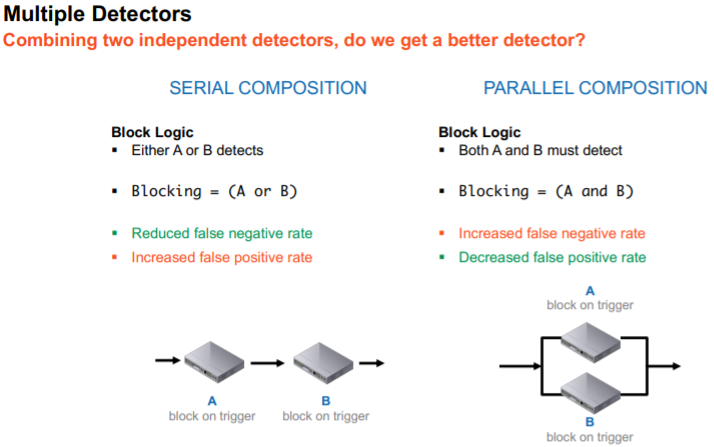
\includegraphics[scale=0.6]{images/911-combine.PNG}
	\caption{Multiple detectors.}
	\label{fig:detect}
\end{figure}



\subsection{Layered Security - Filtering and Protection}

% TODO?


\subsection{Detection Evasion by Design}

\begin{figure}[h]
	\centering
	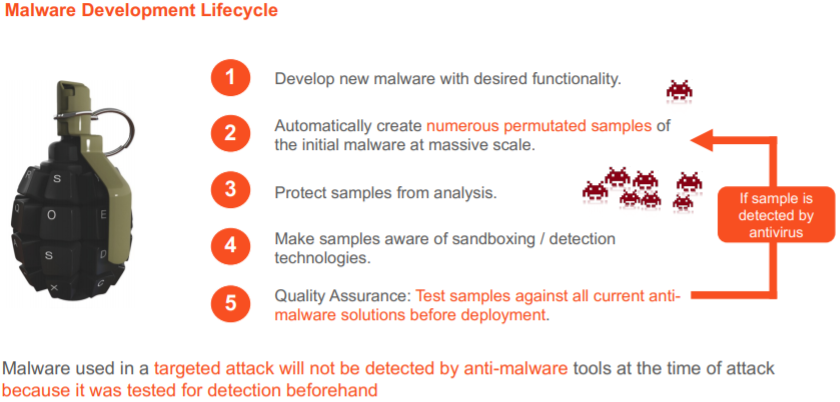
\includegraphics[scale=0.6]{images/911-malware.PNG}
	\caption{Malware development life cycle.}
	\label{fig:malware}
\end{figure}

\paragraph{Step 1: Create Initial Malware}
Create malware core functionality, such as key logger, web-injection, attacks, spreading, communication, etc. by hiring a coder, buying / stealing it or do it yourself.

\paragraph{Step 2: Crypter and Serial Variants}
Encrypt it s.t. signature detection systems and static analysis processes are ineffective. Use different keys to create serial variants / permutations. Encrypt contents of malware executable. Upon execution, only decrypt sections of code on the victim's computer.

\paragraph{Step 3 and 4: Protection Against Debugging}
Use protector technology that detects the use of debuggers or virtualization techniques. If seen, a malware can do different operations (hiding malicious intention or trigger exploitation of virtual environment). %TODO examples

\textbf{Polymorphism techniques:} How to mutate code while keeping the original algorithm intact. Done by manipulating structure of source code of malware by reordering and replacing common programmatic routines. Swapping of equivalent code constructs, changing order of code (registers, instructions, function definitions), inserting noise (redundant code, non-occurring exceptions, functions that are not called), compiler modulation (different compilers can result in different binary code output), etc.

\paragraph{Step 5: Quality Assurance}
Pass malware through many commercial antivirus products (automated). Only use services that do not submit malware samples to vendor! %TODO examples?

%TODO: detection example p.49, watch recording


